\chapter{Introduction - Project Context}\label{ch:context}
\pagestyle{fancy}

{\color{blue}\noindent About 5\% of the paper..\\}
\noindent This chapter will present:

\begin{itemize}
	\item Project context
	\item Specification of the precise domain of the license thesis
\end{itemize}




\section{Project context}\label{sec:context}

\subsection{Subsection title}

Each table used in this document is labeled as Table x.y, where x represents the chapter number, and y shows the table number within the current chapter. Leave a blank line between and after each table, relative to the adjacent paragraphs.
To refer to a table useL ~\ref{tab:nonlin}.

\begin{table}[ht]
	\caption{Results}
	\centering                          % centered table
	\begin{tabular}{|c|c|c|c|}          % 4 centered columns 
		\hline
		Case & Method\#1 & Method\#2 & Method\#3 \\ [0.5ex]   % inserare tabel
		%heading
		\hline                              % horizontal simple line
		1 & 50 & 837 & 970 \\               % table body
		2 & 47 & 877 & 230 \\
		3 & 31 & 25 & 415 \\[1ex]           % [1ex] adds vertical space
		\hline                              
	\end{tabular}
	% titlul tabelului
	\label{tab:nonlin}                % \label{table:nonlin} introduce eticheta folosita pentru referirea tabelului in text; referirea in text se va face cu \ref{table:nonlin}
\end{table}

Each figure used in the document must be referred within the text (ex: in Figure x.y the system components are presented... ) and labeled. The labeling must be as Figure x.y where x represents the chapter number, and y shows the number of the figure within the current chapter. 
Use the following method to refer an image ~\ref{fig:imag}.

\begin{figure}[ht]
	\centering
	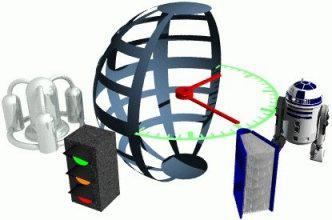
\includegraphics[]{figs/test.jpg}
	\caption{}
	\label{fig:imag}
\end{figure}

Each new chapter starts on a new page.

\vspace{10pt}

\lipsum[1-15]
\newpage